\section[Sequences and Series of Functions]{\hyperlink{toc}{Sequences and Series of Functions}}

\subsection{Motivating Examples}
\begin{nexample}{}{}
    For $m, n \in \NN$, let $p_{n, m} = \frac{m}{n}$. Then, 
    \begin{align*}
        \lim_{m\rightarrow \infty} p_{m, n} = \infty, \quad \linf p_{m, n} = 0
    \end{align*}
    In particular,
    \begin{align*}
        \lim_{m \rightarrow \infty}\linf p_{m, n} = 0, \quad \linf\lim_{m \rightarrow \infty} p_{m, n} = \infty.
    \end{align*}
    Which demonstrates that the order of which limits are taken in can affect the value.
\end{nexample}

\begin{nexample}{}{}
    Define the sequence of functions:
    \begin{align*}
        f_n(x) = \begin{cases}
            1 & x \geq 0
            \\ 1 + nx & -\frac{1}{n} < x < 0
            \\ 0 & x \leq -\frac{1}{n}
        \end{cases}
    \end{align*}
    Since $f_n$ is piecewise linear, it is continuous. However, looking at the $n \rightarrow \infty$ limit, we have:
    \begin{align*}
        \linf f_n(x) = \begin{cases}
            1 & x \geq 0
            \\ 0 & x < 0
        \end{cases}
    \end{align*}
    Which is the right continuous step function, which is evidently discontinuous at $x = 0$. Hence, the limit of continuous functions can be discontinuous. Another way of viewing this problem is:
    \begin{align*}
        \linf \lim_{x \rightarrow 0} f_n(x) = 0, \quad \lim_{x \rightarrow 0} \linf f_n(x) = \text{D.N.E.}
    \end{align*}
    so again we see the order of taking our limits can be important.
\end{nexample}
\begin{figure}[htbp]
    \centering
    \begin{tikzpicture}[scale=1.5]
        \draw[latex-latex, very thick] (-2, 0) -- (2, 0);
        \draw[-latex , very thick] (0, 0) -- (0, 2);
        \draw[<-, thick, blue] (-1.5, 0) -- (-0.5, 0);
        \draw[thick, blue] (-0.5, 0) -- (0, 1);
        \draw[->, thick, blue] (0,1) -- (1.5, 1);
        \draw[] (-0.5, 0) -- (-0.5, -0.15);
        \node[below] at (-0.5, -0.15) {$-\frac{1}{n}$};
    \end{tikzpicture}
    
    
    \caption{Plot of $f_n$ in the above example.}
    \label{fig37}
\end{figure}

\setcounter{rudin}{3}

\begin{example}{}{7.4}
    For $m \in \NN$ and $x \in \RR$, let $f_m(x) = \lim_{n \rightarrow \infty} \left[\cos(m!\pi x)\right]^{2n}$. Since $\abs{\cos(k\pi)} = 1$ if $k \in \ZZ$, we see that $f_m(x) = 1$ when $m! x \in \ZZ$. Conversely, since $\abs{\cos(k\pi)} < 1$ if $k \neq \ZZ$, $f_m(x) = 0$ when $m! x \notin \ZZ$. Some plots of $f_m(x)$ on $[0, 1]$ for $m = 1, 2, 3$ are below as a visualization. We now define $f(x) = \lim_{m \rightarrow \infty} f_m(x)$. If $x = \frac{p}{q} \in \QQ$, then $m! x = \frac{m! p}{q} \in \ZZ$ for $m$ large enough (for $m \geq q$, as the denominator cancells). Therefore, we have that $f(x) = 1$ for $x \in \QQ$. Conversely, if $x \notin \QQ$, then $m! x \notin \ZZ$ for all $m \in \NN$. So, $f_m(x) = 0$ for all $m$, and $f(x) = 0$. Therefore, we have that:
    \begin{align*}
        f(x) = \lim_{m \rightarrow \infty} f_m(x) = \begin{cases}
            1 & x \in \QQ
            \\ 0 & x \notin \QQ
        \end{cases}.
    \end{align*}
    In other words, $f$ is the Dirchlet function. The interesting part is that each of the $f_m(x)$ are Riemann integrable on $[0, 1]$ by Theorem \ref{thm:6.10} (as $f$ has finitely many discontinuities for any $m \in \NN$). However, the limit is not Riemann integrable, as we prove below. Hence, the limit of Riemann integrable functions is not necessarily Riemann integrable.
\end{example}

\begin{figure}[htbp]
    \centering
    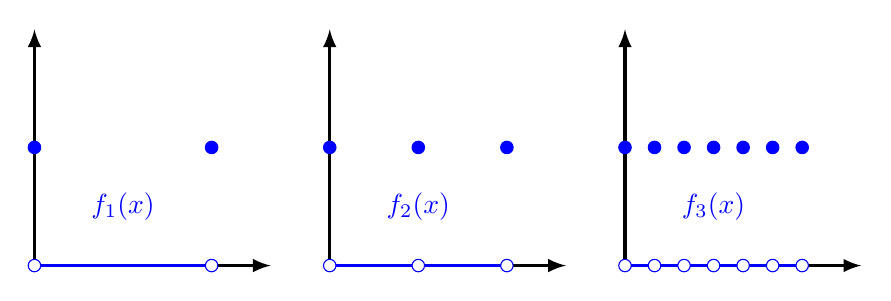
\begin{tikzpicture}[scale = 1.5]
        \draw[-latex, very thick] (0, 0) -- (0, 2);
        \draw[-latex, very thick] (0, 0) -- (2, 0);
        \draw[-latex, very thick] (2.5, 0) -- (2.5, 2);
        \draw[-latex, very thick] (2.5, 0) -- (4.5, 0);
        \draw[-latex, very thick] (5, 0) -- (5, 2);
        \draw[-latex, very thick] (5, 0) -- (7, 0);
        \filldraw[blue] (0, 1) circle (1.5pt);
        \filldraw[blue] (1.5, 1) circle (1.5pt);
        \draw[thick, blue] (0, 0) -- (1.5, 0);
        \draw[blue, fill = white] (0, 0) circle (1.5pt);
        \draw[blue, fill = white] (1.5, 0) circle (1.5pt);
        \node[text = blue] at (0.75, 0.5) {$f_1(x)$};

        \filldraw[blue] (2.5, 1) circle (1.5pt);
        \filldraw[blue] (3.25, 1) circle (1.5pt);
        \filldraw[blue] (4, 1) circle (1.5pt);
        \draw[thick, blue] (2.5, 0) -- (4, 0);
        \draw[blue, fill = white] (2.5, 0) circle (1.5pt);
        \draw[blue, fill = white] (3.25, 0) circle (1.5pt);
        \draw[blue, fill = white] (4, 0) circle (1.5pt);
        \node[text = blue] at (3.25, 0.5) {$f_2(x)$};

        \filldraw[blue] (5, 1) circle (1.5pt);
        \filldraw[blue] (5.25, 1) circle (1.5pt);
        \filldraw[blue] (5.5, 1) circle (1.5pt);
        \filldraw[blue] (5.75, 1) circle (1.5pt);
        \filldraw[blue] (6, 1) circle (1.5pt);
        \filldraw[blue] (6.25, 1) circle (1.5pt);
        \filldraw[blue] (6.5, 1) circle (1.5pt);
        \draw[thick, blue] (5, 0) -- (6.5, 0);
        \draw[blue, fill = white] (5, 0) circle (1.5pt);
        \draw[blue, fill = white] (5.25, 0) circle (1.5pt);
        \draw[blue, fill = white] (5.5, 0) circle (1.5pt);
        \draw[blue, fill = white] (5.75, 0) circle (1.5pt);
        \draw[blue, fill = white] (6, 0) circle (1.5pt);
        \draw[blue, fill = white] (6.25, 0) circle (1.5pt);
        \draw[blue, fill = white] (6.5, 0) circle (1.5pt);
        \node[text = blue] at (5.75, 0.5) {$f_3(x)$};
    \end{tikzpicture}
    \caption{Plot of $f_m(x)$ over the interval $[0, 1]$ for $m = 1, 2, 3$. For $m = 1$, only $x = 0, 1$ satisfy $m! x = x \in \ZZ$. For $m = 2$, we have that $x = 0, \frac{1}{2}, 1$ satisfy $m!x = 2x \in \ZZ$. Finally, for $m = 3$, we have that $x = 0, \frac{1}{6}, \frac{2}{6}, \frac{3}{6}, \frac{4}{6}, \frac{5}{6}, 1$ satisfy $m!x = 6x \in \ZZ$.}
    \label{fig38}
\end{figure}

\noindent We now show that $f$ defined in the above example is not Riemann integrable on $[0, 1]$.

\begin{proof}
    Consider any partition $P$ of $[0, 1]$. Due to the density of rational and irrational numbers in $\RR$ (Theorem \ref{thm:1.20}) we have that $M_i = \sup{f(x): x \in [x_{i-1}, x_i]} = 1$ and $m_i = \inf{f(x): x \in [x_{i-1}, x_i]} = 0$ for all $i$. Therefore, we have that $U(P, f) = \sum_{i=1}^N M_i \Delta x_i = 1$ and $L(P, f) = \sum_{i=1}^N m_i \Delta x_i = 0$ for all partitions $P$. Therefore, $\sup_P U(P, f) = 1$ and $\inf_P L(P, f) = 0$, and we conclude that $f$ is not Riemann integrable on $[0, 1]$.
\end{proof}


\begin{nexample}{}{}
    Define $f_n$ such that:
    \begin{align*}
        f_n(x) = \begin{cases}
            0 & \abs{x} \geq \frac{1}{n}
            \\ n(nx+1) & -\frac{1}{n} < x < 0
            \\ -n(nx+1) & 0 < x < \frac{1}{n}
            \\ 0 & x = 0
        \end{cases}
    \end{align*}
    Then, we have that $f(x) = \linf f_n(x) = 0$ for all $x$.  Furthermore, we have that $\int_{-1}^1 f_n(x)dx = 1$ for all $n$, but $\int_{-1}^1 f(x)dx = 0$. Hence, we have that:
    \begin{align*}
        \linf \int_{-1}^1 f_n(x)dx = 1 \neq 0 = \int_{-1}^1 \linf f_n(x) dx
    \end{align*}
    showing that problems can arise when we interchange the order of an integral with a limit.
\end{nexample}

\begin{figure}[htbp]
    \centering
    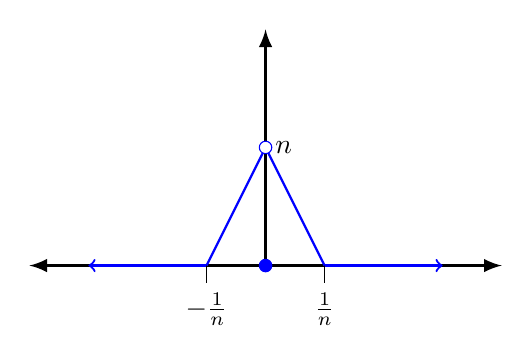
\begin{tikzpicture}[scale=1.5]
        \draw[latex-latex, very thick] (-2, 0) -- (2, 0);
        \draw[-latex , very thick] (0, 0) -- (0, 2);
        \draw[<-, thick, blue] (-1.5, 0) -- (-0.5, 0);
        \draw[thick, blue] (-0.5, 0) -- (0, 1);
        \draw[thick, blue] (0, 1) -- (0.5, 0);
        \draw[->, thick, blue] (0.5, 0) -- (1.5, 0);
        \filldraw[blue] (0, 0) circle (1.5pt);
        \draw[blue, fill = white] (0, 1) circle (1.5pt);
        \node[right] at (0, 1) {$n$};
        \draw[] (-0.5, 0) -- (-0.5, -0.15);
        \node[below] at (-0.5, -0.15) {$-\frac{1}{n}$};
        \draw[] (0.5, 0) -- (0.5, -0.15);
        \node[below] at (0.5, -0.15) {$\frac{1}{n}$};
    \end{tikzpicture}
    
    \caption{Plot of $f_n$ in the above example.}
    \label{fig39}
\end{figure}

\begin{example}{}{7.5}
    Let $f_n(x) = \frac{\sin nx}{\sqrt{n}}$ for $n \in \NN, x \in \RR$. Then, let $f(x) = \linf f_n(x) = 0$ for all $x \in \RR$, so $f'(x) = 0$. However, $f'_n(x) = \frac{1}{\sqrt{n}}n \cos n x = \sqrt{n} \cos n x$ and $\linf \sqrt{n} \cos n x$ does not exist. For example, $f_n'(\pi) = \sqrt{n}(-1)^n$ which is a divergent sequence. So:
    \begin{align*}
        f'(\pi) = \left(\linf f_n\right)'(\pi) = 0 \neq \linf f_n'(\pi)
    \end{align*}
    whcih shows us that problems can arise when interchanging a derivative (which is just a type of limit) with a limit.
\end{example}
\noindent With the above five examples, we have seen examples of bad behaviour that can occur under interchange of limits. Namely:
\begin{enumerate}[1.]
    \item An interchange of the order of limits can change the limiting value for a double sequence.
    \item The limit of a sequence of continuous functions is not necessarily continuous.
    \item The limit of a sequence of Riemann integrable functions is not necessarily Riemann integrable.
    \item The limit of a sequence of Riemann integrals can differ from the Riemann integral of the limit of a sequence.
    \item The limit of a sequence of derivatives can differ from the derivative of a limit of a sequence.
\end{enumerate}

\noindent The good news is that in all of these examples, the sequences we looked at had a ``weak'' form of convergence, where we fix $x$ and then take the $n \rightarrow \infty$ limit. We will now proceed to look at a stronger version of convergence, which looks at ``all $x$ at once'', ensuring that this bad behaviour does not (for the most part) occur.

\subsection{Uniform Convergence}

\setcounter{rudin}{6}
\begin{definition}{Uniform Convergence}{7.7}
    Let $E$ be any set and $f_n: E \mapsto \RR$ or $f_n: E \mapsto \CC$ for $n \in \NN$. Then, $f_n$ \textbf{converges uniformly} to $f$ on $E$ if for all $\e > 0$, there exists $N$ such that $n \geq N$ implies that $\abs{f_n(x) - f(x)} < \e$ for all $x \in E$. 
\end{definition}
\noindent Note the lack of $x$ dependence in the above definition. We give a useful visual intuition of uniform convergence below:

\begin{figure}[htbp]
    \centering
    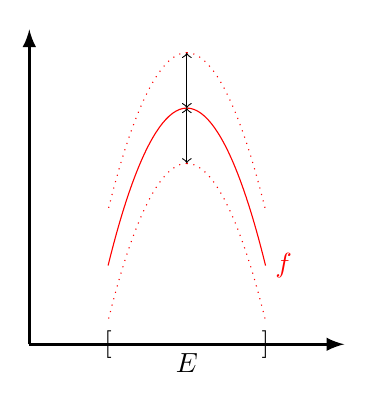
\begin{tikzpicture}[scale=2]
        \draw[-latex, very thick] (0, 0) -- (2, 0);
        \draw[-latex, very thick] (0, 0) -- (0, 2);
        \node[] at (0.5, 0) {$[$};
        \node[] at (1.5, 0) {$]$};
        \node[below] at (1, 0) {$E$};
        \draw[red] (1, 1.5) parabola (0.5, 0.5);
        \draw[red] (1, 1.5) parabola (1.5, 0.5);
        \draw[red, dotted, yshift = 10pt] (1, 1.5) parabola (0.5, 0.5);
        \draw[red, dotted, yshift = 10pt] (1, 1.5) parabola (1.5, 0.5);
        \draw[red, dotted, yshift = -10pt] (1, 1.5) parabola (0.5, 0.5);
        \draw[red, dotted, yshift = -10pt] (1, 1.5) parabola (1.5, 0.5);
        \draw[<->] (1, 1.5) -- (1, 1.15);
        \node[left] at (1, 1.3) {$\e$};
        \draw[<->] (1, 1.5) -- (1, 1.85);
        \node[left] at (1, 1.625) {$\e$};
        \node[right, text = red] at (1.5, 0.5) {$f$};
    \end{tikzpicture}
    
    \caption{Visualization of the intuition behind uniform convergence. If $f_n \rightarrow f$, uniformly, for any $\e > 0$, we can find $N$ such that for $n \geq N$, $f_n(x)$ lies in the $\e$-tube (pictured above) around $f$.}
    \label{fig40}
\end{figure}

\begin{nexample}{}{}
    Let us return to Example \ref{exam:7.5}. We have that:
    \begin{align*}
        \abs{f_n(x) - f(x)} = \abs{\frac{\sin n x}{\sqrt{n}} - 0} \leq \frac{1}{\sqrt{n}}
    \end{align*}
    So taking $n$ large enough such that $\frac{1}{\sqrt{n}} < \e$, we can see that $f_n(x)$ converges uniformly to $f(x) = 0$. Note that this example does show that uniform convergence is \textit{not} sufficient for:
    \begin{align*}
        \lim_{n \rightarrow \infty} f_n' = \left(\lim_{n \rightarrow \infty} f_n \right)'
    \end{align*}
    to hold. We will return to the relation of uniform convergence and differentiation in a later theorem.
\end{nexample}

\begin{nexample}{}{}
    Let us return to our second example from our section on motivating examples. Recall we had:
    \begin{align*}
        f_n(x) = \begin{cases}
            1 & x \geq 0
            \\ 1 + nx & -\frac{1}{n} < x < 0
            \\ 0 & x \leq -\frac{1}{n}
        \end{cases} \quad f(x) = \begin{cases}
            1 & x \geq 0
            \\ 0 & x < 0
        \end{cases}
    \end{align*}
    We then have that:
    \begin{align*}
        f_n(x) - f(x) = \begin{cases}
            1 + nx & -\frac{1}{n} < x < 0
            \\ 0 & \text{otherwise}
        \end{cases}
    \end{align*}
    So for $x = -\frac{1}{2n}$, we have that:
    \begin{align*}
        f_n\left(-\frac{1}{2n}\right) - f\left(-\frac{1}{2n}\right) = 1 + n\left(-\frac{1}{2n}\right) - 0 = \frac{1}{2}
    \end{align*}
    Which will never be less than $\e$ for $\e < \frac{1}{2}$. Hence, we conclude that $f_n$ does not converge uniformly to $f$ on $\RR$. 
\end{nexample}
\begin{figure}[htbp]
    \centering
    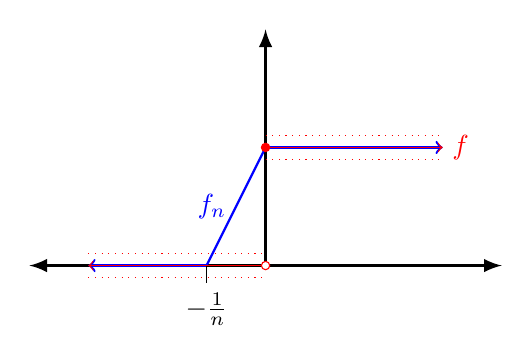
\begin{tikzpicture}[scale=1.5]
        \draw[latex-latex, very thick] (-2, 0) -- (2, 0);
        \draw[-latex , very thick] (0, 0) -- (0, 2);
        \draw[<-, thick, blue] (-1.5, 0) -- (-0.5, 0);
        \draw[thick, blue] (-0.5, 0) -- (0, 1);
        \draw[->, thick, blue] (0,1) -- (1.5, 1);
        \draw[] (-0.5, 0) -- (-0.5, -0.15);
        \node[below] at (-0.5, -0.15) {$-\frac{1}{n}$};
        \draw[->, red] (0, 1) -- (1.5, 1);
        \draw[<-, red] (-1.5, 0) -- (0, 0);
        \draw[red, fill = red] (0, 1) circle (1pt);
        \draw[red, fill = white] (0, 0) circle (1pt);
        \node[left, text = blue] at (-0.25, 0.5) {$f_n$};
        \node[right, text = red] at (1.5, 1) {$f$};
        \draw[dotted, red] (-1.5, 0.1) -- (0, 0.1);
        \draw[dotted, red] (-1.5, -0.1) -- (0, -0.1);
        \draw[dotted, red] (0, 1.1) -- (1.5, 1.1);
        \draw[dotted, red] (0, 0.9) -- (1.5, 0.9);
    \end{tikzpicture}
    
    \caption{Visualization of why the convergence of $f_n \rightarrow f$ in the above example is not uniform. We can see that if we draw a small enough $\e$ tube (i.e. $\e \leq 1$), there is no way to choose $n$ large enough to make all of $f_n(x)$ lie in the tube.}
    \label{fig41}
\end{figure}
\begin{theorem}{Cauchy Criterion for Uniform Convergence}{7.8}
    $f_n$ converges uniformly on $E$ if and only if for all $\e > 0$, thre exists $N$ such that if $m, n \geq N$, then $\abs{f_m(x) - f_n(x)} < \e$ for all $x \in E$. 
\end{theorem}
\noindent Again, note the lack of $x$ dependence in the above theorem.
\begin{nproof}
    $\boxed{\implies}$ Suppose $f_n \rightarrow f$ uniformly on $E$. Then, there exists some $N$ such that for $m, n \geq N$:
    \begin{align*}
        \abs{f_m(x) - f(x)} < \frac{\e}{2}, \quad \abs{f_n(x) - f(x)} < \frac{\e}{2}
    \end{align*}
    for all $x \in E$. Therefore by the triangle inequality, we have that:
    \begin{align*}
        \abs{f_m(x) - f_n(x)} \leq \abs{f_m(x) - f(x)} + \abs{f(x) - f_n(x)} < \frac{\e}{2} + \frac{\e}{2} = \e
    \end{align*}
    Hence $\abs{f_m(x) - f_n(x)} < \e$ for all $x \in E$. 

    $\boxed{\impliedby}$ Let $x \in E$. By assumption, $\set{f_n(x)}_{n \in \NN}$ is a Cauchy sequence, and hence has a limit $f(x)$ (as both $\RR$ and $\CC$, the possible codomains of $f$, are complete). We then let $f(x) = \linf f_n(x)$, so we have pointwise convergence. To see that the convergence is uniform, let $\e > 0$. We know that $\abs{f_m(x) - f_n(x)} < \e$ for $m, n \geq N$ and for all $x$. Then, let $m \rightarrow \infty$. Then, $\abs{f(x) - f_n(x)} \leq \e$. for all $n \geq N$ and all $x \in E$, so the convergence is uniform. \qed
\end{nproof}

\begin{theorem}{}{7.9}
    Suppose $\linf f_n(x) = f(x)$ for $x \in E$, and let:
    \begin{align*}
        M_n = \sup_{x \in E}\abs{f_n(x) - f(x)}
    \end{align*}
    Then, $f_n \rightarrow f$ uniformly on $E$ if and only if $M_n \rightarrow 0$ as $n \rightarrow \infty$.
\end{theorem}
\begin{nproof}
    $\boxed{\implies}$ suppose $f_n \rightarrow f$ uniformly. Then, for any $\e > 0$, there exists some $N \in \NN$ such that for all $n \geq N$ and all $x \in E$:
    \begin{align*}
        \abs{f_n(x) - f(x)} < \e
    \end{align*}
    Since this holds for all $x \in E$, taking the supremum of $\abs{f_n(x) - f(x)}$ we have that:
    \begin{align*}
        \sup_{x \in E}\abs{f_n(x) - f(x)} = M_n \leq \e
    \end{align*}
    We then have that $M_n \leq \e$ for $n \geq N$ for some $N$, and hence $M_n \rightarrow 0$.
    
    $\boxed{\impliedby}$ Suppose that $M_n \rightarrow 0$. Then, for any $\e > 0$, there exists some $N \in \NN$ such that for all $n \geq N$:
    \begin{align*}
        \sup_{x \in E}\abs{f_n(x) - f(x)} = M_n < \e
    \end{align*}
    We then have that for any $x \in E$:
    \begin{align*}
        \abs{f_n(x) - f(x)} \leq \sup_{x \in E}\abs{f_n(x) - f(x)} < \e
    \end{align*}
    so we conclude that $f_n \rightarrow f$ uniformly. \qed
\end{nproof}

\begin{ndef}{: Uniform Convergence of Series}{}
    We say that $\sum_{n = 1}^\infty f_n(x)$ \textbf{converges uniformly} on $E$ if $S_n(x) = \sum_{i=1}^n f_i(x)$ is a uniformly convergent sequence of functions.
\end{ndef}

\begin{theorem}{Weierstrauss M-Test}{7.10}
    Suppose $\abs{f_n(x)} < M_n$ for all $n \geq N_0$ and for all $x \in E$. Suppose also that $\sum_{n = N_0}^\infty M_n < \infty$. Then, $\sum_{n=1}^\infty f_n(x)$ converges uniformly on $E$. 
\end{theorem}
\begin{nproof}
    Let $S_n(x) = \sum_{i=1}^n f_i(x)$. For $n > m \geq N_0$, we have that:
    \begin{align*}
        \abs{S_n(x) - S_m(x)} = \abs{\sum_{i=m+1}^n f_i(x)} \leq \sum_{i=m+1}^n \abs{f_i(x)} \leq \sum_{i=m+1}^n M_i
    \end{align*}
    Let $\e > 0$. Choose $N \geq N_0$ such that $\sum_{i = N+1}^\infty M_i < \e$ (which we can choose as the series converges by assumption). We then have that $\abs{S_n(x) - S_m(x)} < \e$ for all $n > m \geq N$ for all $x \in E$. Hence, $S_n(x)$ converges uniformly on $E$. \qed
\end{nproof}

\begin{theorem}{}{7.11}
    Let $E \subset X$ and $f_n: E \mapsto \RR \text{ or } \CC$, $n \in \NN$. Suppose $f_n \rightarrow f$ uniformly on $E$, and let $x \in E$ (where $x$ is a limit point of $E$). Suppose $\lim_{t \rightarrow x} f_n(t) = A_n$ exists for each $n \in \NN$. Then, $A_n \rightarrow A$ for some $A$ And $\lim_{t \rightarrow x} f(t) = A$. In other words:
    \begin{align*}
        \lim_{t \rightarrow x}\linf f_n(t) = \linf \lim_{t \rightarrow x} f_n(t)
    \end{align*}
    showing that the interchange of limits is valid when we have uniform convergence.
\end{theorem}
\begin{figure}[htbp]
    \centering
    \begin{tikzpicture}[scale=2]
        \draw[-latex, very thick] (0, 0) -- (2, 0);
        \draw[-latex, very thick] (0, 0) -- (0, 2);
        \draw[red] (0, 1) to [ curve through ={(0.5, 1.2)..(1,0.7)..(1.5,1.2)}] (1.7, 1.1);
        \draw[red, dotted, yshift = 5pt] (0, 1) to [ curve through ={(0.5, 1.2)..(1,0.7)..(1.5,1.2)}] (1.7, 1.1);
        \draw[red, dotted, yshift = -5pt] (0, 1) to [ curve through ={(0.5, 1.2)..(1,0.7)..(1.5,1.2)}] (1.7, 1.1);
        \draw[blue] (0, 1.15) to [curve through = {(0.5, 1.1)..(1, 0.8)..(1.5,1.1)}] (1.7, 1);
        \draw[blue, fill = white] (0, 1.15) circle (1pt);
        \node[left, text = blue] at (0, 1.15) {$A_n$};
        \draw[red, fill = white] (0, 1) circle (1pt);
        \node[left, text = red] at (0, 1) {$A$};
        \node[right, text = red] at (1.7, 1.15) {$f$};
        \node[right, text = blue] at (1.7, 0.95) {$f_n$};
    \end{tikzpicture}
    
    \caption{Visualization of Theorem \ref{thm:7.11}, with $E = (0, \infty)$ and $x = 0$. Eventually, the graph of $f_n$ lies in the $\e$ tube around $f$ (no matter how skinny the tube is). But, $A_n$ is being determined by $f_n$ near $0$, so there is nowhere for $A_n$ to go except to the limiting value. That is, $A_n \rightarrow A$ as the $\e$ tube gets compressed.}
    \label{fig42}
\end{figure}

\begin{nproof}
    We first show that $A_n \rightarrow A$ for some $A$. Since $\RR, \CC$ are complete metric spaces, it suffices to show that $\set{A_n}$ is Cauchy. Given $\e > 0$, choose $N$ such that for $m, n \geq N$, $\abs{f_n(t) - f_m(t)} < \e$ for all $t$ (such an $N$ exists by Theorem \ref{thm:7.8}). Letting $t \rightarrow x$, we therefore obtain that $\abs{A_n - A_m} \leq \e$ for all $m, n \geq N$, showing that $\set{A_n}$ is Cauchy. Hence, the sequence converges to some limit $A$. 

    Now, we show that $\lim_{t \rightarrow x}f(t) = A$. We show this by the common ``$\e/3$ argument''. For all $t \in E$ and $n \in \NN$, we have by the triangle inequality that:
    \begin{align*}
        \abs{f(t) - A} \leq \abs{f(t) - f_n(t)} + \abs{f_n(t) - A_n} + \abs{A_n - A} (*)
    \end{align*} 
    Which is a good move, as we know that we can make each of the three terms on the RHS arbitrarily small (they are ``close''). Let $\e > 0$. Since $f_n \rightarrow f$ uniformly, there exists $N_1$ such that $\abs{f(t) - f_n(t)} < \frac{\e}{3}$ for all $n \geq N_1$ and all $t \in E$. Since $A_n \rightarrow A$, there exists some $N_2$ such that $\abs{A_n - A} < \frac{\e}{3}$ for all $n \geq N_2$. Letting $N = \max\set{N_1, N_2}$ and taking $n = N$ in $(*)$, we have that:
    \begin{align*}
        \abs{f(t) - A} < \frac{\e}{3} + \abs{f_N(t) - A_N} + \frac{\e}{3} 
    \end{align*}
    Since $\lim_{t \rightarrow x} f_N(t) = A_N$, we can choose $\delta > 0$ such that $t \in N_{\delta}(x)$ implies $\abs{f_N(t) - A_N} < \frac{\e}{3}$ (Note a subtle point here that this choice of $\delta$ depends on $N$!). Therefore, if $t \in N_{\delta}(x)$, we have that:
    \begin{align*}
        \abs{f(t) - A} < \frac{\e}{3} + \frac{\e}{3} + \frac{\e}{3} = \e
    \end{align*}
    Hence, as $t \rightarrow x$, $f(t) \rightarrow A$. \qed
\end{nproof}

\begin{theorem}{}{7.12}
    Suppose $f_n$ is continuous on $E$ for all $n \in \NN$, and $f_n \rightarrow f$ uniformly on $E$. Then, $f$ is continuous.
\end{theorem}
\begin{nproof}
    Every $f_n$ is continuous at isolated points of $E$, so it suffices to consider limit points $x \in E' \cap E$. For these points, we have that:
    \begin{align*}
        f(x) = \lim_{n \rightarrow \infty}f_n(x) = \linf\lim_{t \rightarrow x} f_n(t) = \lim_{t \rightarrow x} \linf f_n(t) = \lim_{t \rightarrow x} f(t)
    \end{align*}
    Where the third equality (the interchange of the two limits) follows from Theorem \ref{thm:7.11}. We conclude that $f$ is continuous by Theorem \ref{thm:4.6} (as $f(x) = \lim_{t \rightarrow x} f(t)$). \qed
\end{nproof}

\begin{theorem}{}{7.13}
    Suppose $K$ is compact, and:
    \begin{enumerate}
        \item $f_n$ is continuous on $K$ for each $n \in \NN$
        \item $f_n \rightarrow f$ pointwise (that is, for each $x \in K$, $f_n(x) \rightarrow f(x)$) and $f$ is continuous
        \item $f_n(x) \geq f_{n+1}(x)$ for all $x \in K$ and all $n \in \NN$ (note that the opposite inequality also works, just multiply by $-1$).
    \end{enumerate}
    Then, $f_n \rightarrow f$ uniformly on $K$. 
\end{theorem}
\noindent Note that this theorem is not super useful, being that it requires so many specific assumptions; however, we will find that it does have an interesting proof. Before we move to that, let us show some counterexamples for when the assumptions do not hold.

\begin{nexample}{}{}
    Let $K = [-1, 0)$, and define:
    \begin{align*}
        f_n(x) = \begin{cases}
            0 & -1 \leq x \leq -\frac{1}{n}
            \\ 1 + nx & -\frac{1}{n} < x < 0
        \end{cases}
    \end{align*}
    We then have that $f_n$ is continuous on $K$, that $f_n \rightarrow 0$ pointwise on $K$, that $f$ is continuous (the zero function), and $f_n$ is decreasing with $n$. However, we note that $f_n$ does not converge uniformly to $f$ on $K$, with points close to zero being problem points (for example, take $x = -\frac{1}{2n}$, and then $f_n(x) - f(x) = \frac{1}{2}$ for all $n$). We note that $K$ is \textit{not} compact, showing the importance of compactness of the domain in the above Theorem.
\end{nexample}
\begin{figure}[htbp]
    \centering
    \begin{tikzpicture}[scale=1.5]
        \draw[latex-latex, very thick] (-2, 0) -- (2, 0);
        \draw[-latex , very thick] (0, 0) -- (0, 2);
        \draw[thick, blue] (-1.5, 0) -- (-0.5, 0);
        \draw[thick, blue] (-0.5, 0) -- (0, 1);
        \draw[blue, fill = white] (0, 1) circle (1pt);
        \draw[] (-1.5, 0) -- (-1.5, -0.15);
        \draw[blue, fill = blue] (-1.5, 0) circle (1pt);
        \draw[] (-0.5, 0) -- (-0.5, -0.15);
        \node[below] at (-0.5, -0.15) {$-\frac{1}{n}$};
        \node[below] at (-1.5, -0.15) {$-1$};
        \node[right] at (0, 1) {$1$};
    \end{tikzpicture}
    
    \caption{Plot of $f_n$ on $K = [-1, 0)$ from the above example.}
    \label{fig43}
\end{figure}

\begin{nexample}{}{}
    Let $K = [0, 1]$, and define:
    \begin{align*}
        f_n(x) = \begin{cases}
            2nx & 0 \leq x < \frac{1}{2n}
            \\ 2 - 2nx & \frac{1}{n} \leq x \leq \frac{1}{n}
            \\ 0 & \frac{1}{n} < x \leq 1
        \end{cases}
    \end{align*}
    We then have that $f_n$ is continuous, $f_n \rightarrow f = 0$ pointwise (which is continuous), and $K$ is compact. However, $f_n$ does not converge to $f$ uniformly. In this case, condition (c) of the above Theorem fails; $f_n$ is not monotonic in $n$.
\end{nexample}
\begin{figure}[htbp]
    \centering
    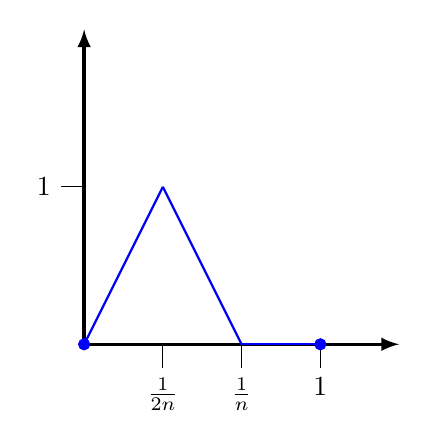
\begin{tikzpicture}[scale=2]
        \draw[-latex, very thick] (0, 0) -- (2, 0);
        \draw[-latex, very thick] (0, 0) -- (0, 2);
        \draw[] (1, 0) -- (1, -0.15);
        \draw[blue, thick] (0, 0) -- (0.5, 1);
        \draw[blue, thick] (0.5, 1) -- (1, 0);
        \draw[blue, thick] (1, 0) -- (1.5, 0);
        \draw[] (1.5, 0) -- (1.5, -0.15);
        \draw[blue, fill = blue] (1.5, 0) circle (1pt);
        \draw[blue, fill = blue] (0, 0) circle (1pt);
        \draw[] (0, 1) -- (-0.15, 1);
        \node[left] at (-0.15, 1) {$1$};
        \node[below] at (1.5, -0.15) {$1$};
        \draw[] (0.5, 0) -- (0.5, -0.15);
        \node[below] at (0.5, -0.15) {$\frac{1}{2n}$};
        \node[below] at (1, -0.15) {$\frac{1}{n}$};
    \end{tikzpicture}
    
    \caption{Plot of $f_n$ on $K = [0, 1]$ from the above example.}
    \label{fig44}
\end{figure}

\begin{nproof}
    Let $g_n = f_n - f$. We can then see that:
    \begin{enumerate}
        \item $g_n$ is continuous (the difference of two continuous functions is continuous by Theorem \ref{thm:4.9})
        \item $g_n \rightarrow 0$ pointwise for all $x \in K$
        \item $g_n \geq g_{n+1} \geq 0$ for all $x \in K$.
    \end{enumerate}
    The goal will be to show that $g_n \rightarrow 0$ uniformly on $K$. We will use the finite intersection property of compact sets to show this. Let $\e > 0$. We will show that there exists $N$ such that $0 \leq g_n(x) < \e$ for all $n \geq N$ and for all $x \in K$. Note that it suffices to show that $g_N(x) < \e$ for some $N$, as $g$ is monotone decreasing in $n$. Define $K_n = g_{n}^{-1}([\e, \infty))$ (i.e. the set of ``bad $x$s''). We are done if we are able to show that there exists a $N$ with $K_N = \emptyset$. Since $g_n$ is conitnuous, $K_n$ is closed as $[\e, \infty)$ is closed. Since $K_n \subset K$, $K$ is therefore compact as a closed subset of a compact set (Theorem \ref{thm:2.35}). Additionally, we have that $K_{n+1} \subset K_n$, as $g_{n+1} \geq \e$ implies that $g_n \geq \e$. Since $g_n \rightarrow 0$ pointwise, given $x \in K$, there exsits $N_x$ such that $x \notin K_n$ for all $n \geq N_x$ (as $g_n(x) < \e$ for large enough $n$). We therefore have that $x \notin \bigcap_n K_n$ for all $x \in K$. Then, applying the corollary to Theorem \ref{thm:2.36}, we obtain that $K_N$ is empty. This means that for this $N$, $g_N^{-1}([\e, \infty)) = \emptyset$, and hence $g_N^{-1}([0, \e]) = K$, which is to say that $0 \leq g_n(x) < \e$ for all $x \in K$. \qed
\end{nproof}

\begin{definition}{$\C(X)$ and the Supremum Norm}{7.14}
    For a metric space $X$, define:
    \begin{align*}
        \C(X) = \set{f: X \mapsto \CC \text{ such that $f$ is bounded and continuous.}}
    \end{align*}
    The \textbf{supremum norm} of $f \in \C(X)$ is then defined as $\norm{f} = \sup_{x \in X}\abs{f(x)}$. We claim that $\norm{f - g}$ defines a metric on $\C(X)$, and we prove this assertion below. Thus, we have that:
    \begin{align*}
        f_n \rightarrow f \text{ uniformly} &\iff \forall \e > 0, \exists N \text{ such that } \abs{f_n(x) - f(x)} < \e \; \forall n \geq N \text{ and } \forall x \in X
        \\ &\iff \forall \e > 0, \exists N \text{ such that } \norm{f_n(x) - f(x)} < \e \; \forall n \geq N
        \\ &\iff f_n \rightarrow f \text{ in the metric space $\C(X)$}
    \end{align*}
    We have hence ``metrized'' uniform convergence.
\end{definition}
\begin{ntheorem}{}{}
    $\norm{f - g}$ defines a metric on $\C(X)$.
\end{ntheorem}
\begin{nproof}
    We recall the three properties of a metric as per Definition \ref{def:2.15}:
    \begin{enumerate}
        \item $d(f, g) = 0 \iff f = g$
        \item $d(f, g) = d(g, f)$
        \item $d(f, g) \leq d(f, h) + d(h, g)$
    \end{enumerate}
    We now show that $\norm{f - g}$ satisfies these three properties.
    \begin{enumerate}
        \item $\norm{f - g} = 0$ means that $0 = \sup_{x \in X}\abs{f(x) - g(x)} \implies \abs{f(x) - g(x)} = 0$ for all $x$, hence $f(x) = g(x)$. 
        \item $\norm{f - g} = \sup_{x \in X}\abs{f(x) - g(x)} = \sup_{x \in X}\abs{g(x) - f(x)} = \norm{g - f}$
        \item We have that $\abs{f(x) - g(x)} \leq \abs{f(x) - h(x)} + \abs{h(x) - g(x)}$ for all $x \in X$, so $\norm{f - g} \leq \norm{f - h} + \norm{h - g}$. \qed
    \end{enumerate}
\end{nproof}

\noindent Note that sometimes $\norm{f}$ is written as $\norm{f}_\infty$ as it is the $n \rightarrow \infty$ limit of the $L_p$ norm. See HW3Q3 for the proof that the supremum norm is the limit of the $L_p$ norm. 

\begin{theorem}{}{7.15}
    $\C(X)$ is a complete metric space (every Cauchy sequence in $\C(X)$ has a limit in $\C(X)$).
\end{theorem}
\begin{nproof}
    Let $\set{f_n}$ be a Cauchy sequence in $\C(X)$. Then, given $\e > 0$, $\exists N$ such that $m, n \geq N$ implies $\norm{f_m - f_n} = \sup_{x \in X}\abs{f_m(x) - f_n(x)} < \e$. By the Cauchy criterion (Theorem \ref{thm:7.8}), $f_n \rightarrow f$ for some $f$. What is left to show is that $f \in \C(X)$. $f$ is continuous as it is the uniform limit of continuous functions (Theorem \ref{thm:7.12}). Additionally, $f$ is bounded as there exists $N_0$ such that $\abs{f(x) - f_{N_{0}}(x)} < 1$ for all $x$, and hence $\abs{f(x)} \leq \abs{f_{N_0}(x)} + \abs{f(x) - f_{N_0}(x)} \leq M_0 + 1$ for all $x$ where $M_0$ is the bound on $f_{N_0}(x)$ that exists as $f_{N_0} \in \C(X)$. As $f$ is continuous and bounded, we conclude that $f \in \C(X)$. \qed
\end{nproof}

\subsection{Uniform Convergence and Integration}
\begin{theorem}{}{7.16}
    Suppose $f_n \in \R_{\alpha}[a, b]$ for all $n \in \NN$ and that $f_n \rightarrow f$ uniformly on $[a, b]$. Then, $f \in \R_{\alpha}[a, b]$, and:
    \begin{align*}
        \linf \int_{a}^b f_n d\alpha = \int_a^b f d\alpha
    \end{align*}
\end{theorem}

\newpage
\noindent In other words, the above Theorem tells us that we can interchange the integral with the limit if the sequence is uniformly convergent. Compare this to our earlier example with pointwise convergence, where such an interchange was not possible (as it yielded different values).

\begin{nproof}
    First, we show that $f \in \R_{\alpha}[a, b]$. Let $\e > 0$. Since $f_n \rightarrow f$ uniformly, there exists $N$ such that $\abs{f_n(X) - f(x)} < \e$ if $n \geq N$ for all $x \in [a, b]$. So, $f_n(x) - \e < f(x) < f_n(x) + \e$. Hence,
    \begin{align*}
        \lint{a}{b}(f_n - \e)d\alpha \leq \lint{a}{b}fd\alpha \leq \uint{a}{b} fd\alpha \leq \uint{a}{b}(f_n + \e)d\alpha 
    \end{align*}
    Since $f_n \pm \e \in \R_{\alpha}[a, b]$, we have that:
    \begin{align*}
        \int_{a}^b (f_n - \e)d\alpha \leq \lint{a}{b}fd\alpha \leq \uint{a}{b} fd\alpha \leq \int_a^b(f_n + \e)d\alpha 
    \end{align*}
    Therefore:
    \begin{align*}
        0 \leq \uint{a}{b} fd\alpha - \lint{a}{b} fd\alpha \leq \int_a^b 2\e d\alpha \implies \uint{a}{b} fd\alpha - \lint{a}{b} fd\alpha \leq 2\e(\alpha(b) - \alpha(a))
    \end{align*}
    Since $\e$ is arbitrary, we have that $\uint{a}{b} fd\alpha = \lint{a}{b} fd\alpha$ and hence $f \in \R_\alpha[a, b]$.

    Next, we show that $\linf \int_{a}^b f_n d\alpha = \int_a^b f d\alpha$. To do this, we show that $\abs{\int_a^b fd\alpha - \int_a^bf_nd\alpha}$ goes to 0 as $n \rightarrow \infty$. We have that:
    \begin{align*}
        \abs{\int_a^b fd\alpha - \int_a^bf_nd\alpha} = \abs{\int_a^b (f - f_n)d\alpha} \leq \int_a^b\abs{f - f_n}d\alpha \leq \int_a^b \e d\alpha = \e(\alpha(b) - \alpha(a))
    \end{align*}
    Where in the first equality we use Linearity (Theorem \ref{thm:6.12}), the first inequality we apply Theorem \ref{thm:6.13}, and in the second inequality, we use that for any $\e > 0$, there exists $N$ such that $\abs{f - f_n} < \e$ for $n \geq N$. Since $\e$ is arbitrary, we conclude that $\linf \int_{a}^b f_n d\alpha = \int_a^b f d\alpha$. \qed
\end{nproof}

\begin{ncorollary}{}{}
    If $f_n \in \R_\alpha[a, b]$ and $f(x) = \sum_{n=1}^\infty f_n(x)$ converges uniformly on $[a, b]$, then $\int_a^b fd\alpha = \sum_{n=1}^\infty \int_a^b f_n d\alpha$. That is to say, the infinite series and the integral can be interchanged.
\end{ncorollary}

\begin{nproof}
    Let $S_n(x) = \sum_{i=1}^n f_i(x)$. Then, $S_n(x) \rightarrow f(x)$ uniformly by assumption, so:
    \begin{align*}
        \int_a^b fd\alpha = \linf \int_a^b s_n d\alpha = \linf \sum_{i=1}^n \int_a^b f_i d\alpha = \sum_{i=1}^\infty \int_a^b f_i d\alpha
    \end{align*}
    Where the first equality follows from the previous theorem, and the second equality follows from the fact that a finite sum and integral can be interchanged by Linearity. \qed
\end{nproof}

\subsection{Uniform Convergence and Differentiation}
Recall Example \ref{exam:7.5}, where we looked at the sequence of functions $f_n(x) = \frac{\sin n x}{\sqrt{n}}$. We showed that $f_n \rightarrow 0$ uniformly on $\RR$, but we found in the example that $f_n'(x)$ does \emph{not} converge. We are therefore motivated to find a condition that if a function converges and is differentiable, then $f_n'$ converges.

As a point of notation, note that for $a < b$ we denote $\int_b^a f d\alpha = -\int_a^b fd\alpha$. 

\begin{theorem}{}{7.17}
    Suppose:
    \begin{enumerate}
        \item $f_n$ is differentiable on $[a, b]$;
        \item $\exists x_0 \in [a, b]$ such that $f_n(x_0)$ converges as $n \rightarrow \infty$;
        \item $f_n'$ converges uniformly on $[a, b]$. 
    \end{enumerate}
    Then, there exists $f$ such that $f_n \rightarrow f$ uniformly on $[a, b]$, and:
    \begin{align*}
        \linf f_n'(x) = f'(x) \; \forall x \in [a, b]
    \end{align*}
\end{theorem}
\noindent A couple remarks before we move to the proof. First, we note that hypothesis (b) seems strange; why would we require convergence $f_n$ at a single point? This has to do with the fact that in differentiating, we lost our constants. For example, let $f_n(x) = n$ as the simplest example. In this case, we have that $f_n$ is differentiable everywhere (with derivative zero everywhere on $[a, b]$) and that $gfn'$ uniformly converges (it is just the sequence of the zero function). However, $f_n$ does not even converge!

Note that we can and will assume that $f_n(x_0) \rightarrow 0$ at the specified $x_0$; if this is not true, we can simply replace $f_n(x)$ by $f_n(x) - f_n(x_0)$.

\begin{nproof}
    The proof of the above theorem is not so trivial. We will therefore prove a weaker theorem. Namely, we add a fourth hypothesis (d) that $f_n'$ is continuous on $[a, b]$. The proof of the stronger/original theorem can be found in Rudin.
    
    First, by (c) there exists a $g$ such that $f_n' \rightarrow g$ uniformly on $[a, b]$ (and also on any subinterval of $[a, b]$). Furthermore, by (d) and Theorem \ref{thm:7.12}, $g$ is continuous. 
    
    Next, applying Theorem \ref{thm:7.16} (to either $[x_0, x]$ or $[x, x_0]$) we have that:
    \begin{align*}
        \int_{x_0}^x f_n'(t) \rightarrow \int_{x_0}^x g(t) dt = f(x)
    \end{align*}
    Then applying the Fundamental theorem of calculus (Theorem \ref{thm:6.21}), we have $f_n(x) - f_n(x_0) \rightarrow f(x) \text{ and } f'(x) = g(x)$. But we also assume that $f_n(x_0) \rightarrow 0$, so $f_n(x) \rightarrow f(x)$ and $f_n'(x) \rightarrow g(x) = f'(x)$. So, we have shown pointwise convergence of $f_n$ to $f$! We have obtained that $\linf f_n'(x) = f'(x)$ for all $x \in [a, b]$. Finally, we show $f_n \rightarrow f$ uniformly on $[a, b]$. We have that:
    \begin{align*}
        \abs{f(x) - f_n(x)} = \abs{\int_{x_0}^x g(t)dt - \int_{x_0}^x f_n'(t) dt + f_n(x_0)} &\leq \int_{x_0}^x \abs{g(t) - f_n'(t)}dt + \abs{f_n(x_0)}
        \\ &< \int_{x_0}^x \frac{\e}{2(b-a)}dt + \frac{\e}{2} \leq \frac{\e}{2(b-a)}(b-a) + \frac{\e}{2} = \e
    \end{align*}
    Where we apply Theorem \ref{thm:6.13} for the first inequality, the fact that $f_n'(t) \rightarrow g$ and $f_n(x_0) \rightarrow 0$ in the second last inequality, and Theorem \ref{thm:6.12}(d) in the last inequality. \qed
\end{nproof}

\begin{theorem}{}{7.18}
    There exists a continuous function $f: \RR \mapsto \RR$ such that $f'(x)$ does not exist for any $x \in \RR$.
\end{theorem}

\noindent The proof of the above theorem will follow by the construction of an ``infinitely spiky'' real function. Though this might seem like a very pathological counterexample, there are actually many examples of non-differentiable phenomena in mathematics. Looking at the field of probability, we find that brownian motion, brownian maps, and discrete exploration processes (to name a few) all have this property. A visualization of the brownian map, as well as other beautiful probability pictures can be found here \url{https://secure.math.ubc.ca/Links/Probability/pages/pic_gallery.html}.

\begin{figure}[htbp]
    \centering
    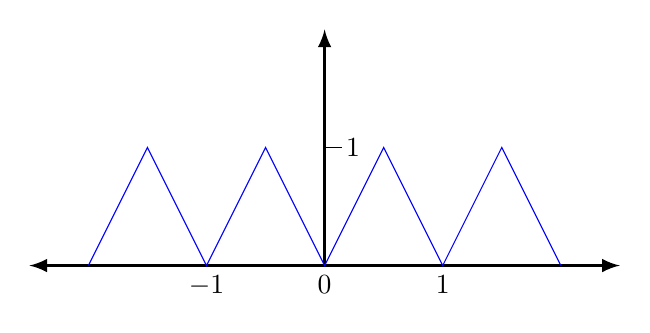
\begin{tikzpicture}[scale=1.5]
        \draw[-latex, very thick] (0, 0) -- (0, 2);
        \draw[latex-latex, very thick] (-2.5, 0) -- (2.5, 0);
        \draw[blue] (-2, 0) -- (-1.5, 1) -- (-1, 0) -- (-0.5, 1) -- (0, 0) -- (0.5, 1) -- (1, 0) -- (1.5, 1) -- (2, 0);
        \draw[] (0, 1) -- (0.15, 1);
        \draw[right] node at (0.1, 1) {$1$};
        \draw[below] node at (0, 0) {$0$};
        \draw[below] node at (1, 0) {$1$};
        \draw[below] node at (-1, 0) {$-1$};


    \end{tikzpicture}
    \caption{Plot of the $\phi$ function defined in the proof of Theorem \ref{thm:7.18}.}
    \label{fig45}
\end{figure}

\begin{figure}[htbp]
    \centering
    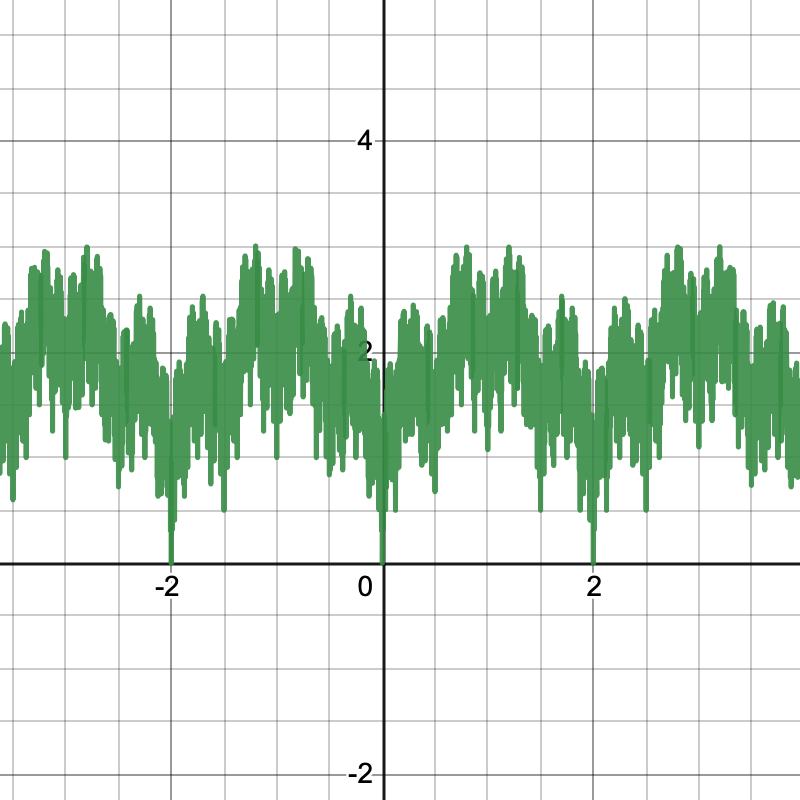
\includegraphics[scale=0.25]{Images/7-18-graph.png}
    
    \caption{Desmos visualization of the nowhere-differentiable $f$ constructed in the proof of Theorem \ref{thm:7.18}. Note that a partial sum $(N = 10)$ of the series that $f$ is defined to be is shown, as the infinite series is impossible to plot. Readers can play around the function with themselves at \url{https://www.desmos.com/calculator/onhkmblgo6}. There is a notion that $f$ is ``infinitely spiky'', no matter how much one is to zoom into the above graph.}
    \label{fig46}
\end{figure}

\begin{nproof}
    Define $\phi: \RR \mapsto \RR$ by $\phi(x) = \abs{x}$ for $-1 \leq x \leq 1$ and $\phi(x + 2) = \phi(x)$ for all $x \in \RR$. (See figure \ref{fig45} above). Then, $\phi$ is continuous; moreover, it is Lipschiz continuous, with $\abs{\phi(s) - \phi(t)} \leq \abs{s - t}$ for all $s, t \in \RR$ (with equality where there are no integers between $s, t$). Define $f(x) = \sum_{n=0}^\infty \left(\frac{3}{4}\right)^n \phi(4^nx)$. The series converges uniformly on $\RR$ by Theorem \ref{thm:7.10}, since $0 \leq \left(\frac{3}{4}\right)^n \phi(4^nx) \left(\frac{3}{4}\right)^n$ and $\sum_n\left(\frac{3}{4}\right)^n$ converges (it is a geometric series with $r < 1$). Hence, $f$ is continuous as it is a uniform limit of a continuous function (Theorem \ref{thm:7.12}). We now prove that $f'(x)$ does not exists for any $x \in \RR$; let us then fix $x$. It suffices to find $\delta_m \rightarrow 0$ such that:
    \begin{align*}
        \abs{\frac{f(x + \delta_m) - f(x)}{\delta_m}} \rightarrow \infty \text{ as } m \rightarrow \infty.
    \end{align*}
    We then choose $\delta_m = \pm \frac{1}{2}\frac{1}{4^m}$. We choose the sign of $\delta_m$ depending on the choice of $x$ as follows. At most one of $(4^m x - \frac{1}{2}, 4^mx)$ and $(4^mx, 4^mx + \frac{1}{2})$ contains an integer. We choose the sign such that no integer lies between $4^m x$ and $4^m(x + \delta_m)$. Note that we may choose a differnet sign for each $m$. 
    
    Next, we make the observation that $\abs{\phi(4^m(x + \delta_m)) - \phi(4^mx)} = 4^mx$; this holds as for the difference between two $\phi(x)$ values at two points without an integer between them is just the difference between the $x$ values. Looking back at our definition of $\delta_m$, we then see that $\abs{\phi(4^m(x + \delta_m)) - \phi(4^mx)} = \frac{1}{2}$.

    Furthermore, we see that if $n > m$, we have that $\phi(4^n(x + \delta_m)) - \phi(4^nx \pm \frac{1}{2}4^{n-m}) = \phi(4^nx)$ as $\frac{1}{2}4^{n-m}$ is an even integer and $\phi$ is 2-periodic. This leads us to conclude that $\phi(4^n(x + \delta_m)) - \delta(4^nx) = 0$ if $n > m$. Given $m$, then define:
    \begin{align*}
        \gamma_n = \frac{\phi(4^n(x + \delta_m)) - \delta(4^nx)}{\delta_m}
    \end{align*}
    Then, $\gamma_n = 0$ if $n > m$, $\abs{\gamma_m} = \abs{\frac{4^m\delta_m}{\delta_m}} = \abs{4^m} =4^m$, and if $0 \leq n < m$, $\abs{\gamma_n} \leq \frac{1}{\delta_m}\abs{4^n(x + \delta_m) - 4^nx} = \frac{1}{\abs{\delta_m}}\abs{4^n\delta_m} = 4^n$. Finally, we have that:
    \begin{align*}
        \abs{\frac{f(x + \delta_m) - f(x)}{\delta_m}} = \abs{\sum_{n=0}^\infty \left(\frac{3}{4}\right)^n\gamma_m} = \abs{\sum_{n=0}^m \left(\frac{3}{4}\right)^n\gamma_m} &\geq \left(\frac{3}{4}\right)^m\abs{\gamma_m} - \sum_{n=0}^{m-1}\left(\frac{3}{4}\right)^n\abs{\gamma_n}
        \\ &\geq \left(\frac{3}{4}\right)^m4^m - \sum_{n=0}^{m-1}\left(\frac{3}{4}\right)^n4^n
        \\ &= 3^m - \sum_{n=1}^{m-1}3^n
        \\ &= 3^m - \frac{3^m - 1}{3 - 1}
        \\ &= \frac{1}{2}(3^m + 1)
    \end{align*}
    Where the second equality follows as all terms $n > m$ are zero, the first inequality follows by the reverse triangle inequality, the second inequality follows by the bounds on $\abs{\gamma_n}$, and the third-to-last equality is the geometric sum formula. As $m \rightarrow \infty$, the difference quotient goes to infinity, and we therefore conclude that $f$ is differentiable nowhere. \qed
\end{nproof}

\subsection{Equicontinuituous Families of Functions}
\setcounter{rudin}{21}
\begin{definition}{Equicontinuity}{7.22}
    A family $\mathcal{F}$ of functions on $E$ (that is, a possibly finite, countable, or uncountable set of functions on $E$) is \textbf{equicontinuous} on $E$ if for every $\e > 0$, there exists $\delta > 0$ such that if $f \in \mathcal{F}$ and $x, y \in E$ with $d(x, y) < \delta$, then $\abs{f(x) - f(y)} < \e$. Note that the functions $f \in \mathcal{F}$ are either real or complex valued.
\end{definition}
\noindent The above definition of equicontinuity is essentially an even stronger version of uniform continuity; the $\delta$ works not just for all $x$ and $y$ for a single $f$, but for all $x$ and $y$ for all of the $f$s in $\mathcal{F}$. If $\mathcal{F} = \set{f}$, then this is just uniform continuity.

\begin{ntheorem}{}{}
    \begin{enumerate}
        \item If a family $\mathcal{F}$ of functions on $E$ is equicontinuous, then every $f \in \mathcal{F}$ is uniformly continuous on $E$.
        \item Any finite family $\mathcal{F} = \set{f_1, \ldots f_n}$ of uniformly continuous functions on $E$ is equicontinuous.
    \end{enumerate}
\end{ntheorem}
\begin{nproof}
    \begin{enumerate}
        \item The claim follows immediately from the definition.
        \item Let $\e > 0$. Then, by the uniform continuity of each $f_i \in \mathcal{F}$, there exists $\delta_i$ such that if $d(x, y) < \delta_i$, then $\abs{f_i(x) - f_i(y)} < \e$. Taking $\delta = \min{\delta_1, \ldots, \delta_n}$, we have that for any $f \in \mathcal{F}$, if $d(x, y) < \delta$ then $\abs{f(x) - f(y)} < \e$. Hence $\mathcal{F}$ is equicontinuous. \qed
    \end{enumerate}
\end{nproof}

\begin{nexample}{}{}
    Let $\mathcal{F} = \set{f_1, f_2, \ldots}$ with $f_n(x) = \frac{\sin (nx)}{\sqrt{n}}$ for $x \in [0, 1] \in E$. Then, $\mathcal{F}$ is equicontinuous.
\end{nexample}
\begin{nproof}
    We have that $\abs{f_n(x) - f_n(y)} = \frac{1}{\sqrt{n}}\abs{\sin(nx) - \sin(ny)} \leq \frac{2}{\sqrt{n}}$ for all $x, y \in E$. Let $\e > 0$. Choose $N$ such that $\frac{2}{\sqrt{n}} < \e$ if $n > N$. Since the remaining $f_n$ (i.e. $\set{f_1, \ldots, f_{n}}$) are a finite collection of uniformly continuous functions (they are uniformly continuous by Theorem \ref{thm:4.19}, as they continuous functions on a closed and bounded interval), by the above theorem, $\set{f_1, \ldots f_{n}}$ is equicontinuous. So, there exists a $\delta$ such that for $n \geq N$ and $\abs{x - y} < \delta$, $\abs{f_n(x) - f_n(y)} < \e$. We then have that for any $n \in \NN$ and for any $x, y \in E$ with $\abs{x - y} < \delta$, then $\abs{f_n(x) - f_n(y)} < \e$. We conclude that $\mathcal{F}$ is equicontinuous. \qed
\end{nproof}

\begin{ntheorem}{ (Problem 7.16)}{}
    Let $\set{f_n}$ be an equicontinuous sequnece of functions such that $f_n: K \mapsto \CC$ with $K$ compact. Suppose there is a pointwise limit $f(x) = \linf f_n(x)$ that exists for all $x \in K$. Then, $f_n \rightarrow f$ uniformly on $K$.
\end{ntheorem}
\begin{nproof}
    We use an ``$\frac{\e}{3}$ argument''. Let $\e > 0$. Then, choose $\delta > 0$ such that $\abs{f_n(x) - f_n(y)} < \frac{\e}{3}$ for all $n$ and for all $x, y$ such that $d(x, y) < \delta$ (such a choice is possible by the equicontinuity of the sequence). Take an open cover of $K$ by considering the set of neighbourhoods of radius $\delta$ around every point $x \in K$. Since $K$ is compact, the open cover $\set{N_{\delta}(x): x \in K}$ has a finite subcover $\set{N_\delta(x_1), \ldots, N_\delta(x_k)}$. Thus, given $x \in K$, there exists $x_j$ such that $x \in N_\delta(x_j)$ and hence $d(x_j, x) < \delta$. Therefore by the triangle inequality:
    \begin{align*}
        \abs{f_n(x) - f_m(x)} &\leq \abs{f_n(x) - f_n(x_j)} + \abs{f_n(x_j) - f_m(x_j)} + \abs{f_m(x_j) - f_m(x)}
        \\ &< \frac{\e}{3} + \abs{f_n(x_j) - f_m(x_j)} + \frac{\e}{3}
    \end{align*}
    where the last inequality follows from the equicontinuity. For each $i \in \set{1, \ldots k}$, we know that $\set{f_n(x_j)}$ is a convergent sequence as $f_n$ converges pointwise by assumption. Hence, it is a Cauchy sequence. Therefore, there exists a $N_i$ such that $m, n \geq N_i$ implies $\abs{f_n(x_i) - f_m(x_i)} < \frac{\e}{3}$. Take $N = \max{N_1, \ldots, N_k}$. Then, we have that $m, n \geq N$ implies:
    \begin{align*}
        \abs{f_n(x) - f_m(x)} < \frac{\e}{3} + \frac{\e}{3} + \frac{\e}{3} = \e.
    \end{align*}
    So, $f_n$ satisfies the Cauchy criterion for uniform convergence, and hence $\set{f_n}$ converges uniformly on $K$. \qed
\end{nproof}

\setcounter{rudin}{23}

\begin{theorem}{}{7.24}
    If $f_n: K \mapsto \CC$ is continuous, $K$ is compact, and $f_n \mapsto f$ uniformly on $K$, then $\set{f_n}$ is equicontinuous.
\end{theorem}
\begin{nproof}
    We again use an ``$\frac{\e}{3}$ argument''. Let $\e > 0$. Since $f_n \rightarrow f$ uniformly, we have that there exists $N$ such that $m, n \geq N$ implies $\abs{f_n(x) - f_m(x)} < \frac{\e}{3}$ for all $x \in K$. Also, since $K$ is compact, each $f_i$ is unformly continuous, so $\set{f_1, \ldots f_N}$ is equicontinuous for any $N \in \NN$ (as it is a finite set of uniformly continuous functions). Hence, there exists $\delta > 0$ such that $\abs{f_i(x) - f_i(y)} < \frac{\e}{3}$ if $d(x, y) < \delta$ and $i \leq N$. Finally, for $n > N$, we habe that:
    \begin{align*}
        \abs{f_n(x) - f_n(y)} \leq \abs{f_n(x) - f_N(x)} + \abs{f_N(x) - f_N(y)} + \abs{f_N(y) - f_n(y)} < \frac{\e}{3} + \frac{\e}{3} + \frac{\e}{3} = \e
    \end{align*}
    where the first/third $\frac{\e}{3}$s come from uniform convergence and the second from the equicontinuity. We conclude that $\set{f_n}$ is equicontinuous. \qed
\end{nproof}

\begin{nexample}{}{}
    We here discuss a set of functions which is not equicontinuous, by returning to a prior example. Let $K = [0, 1]$, and define:
    \begin{align*}
        f_n(x) = \begin{cases}
            2nx & 0 \leq x < \frac{1}{2n}
            \\ 2 - 2nx & \frac{1}{n} \leq x \leq \frac{1}{n}
            \\ 0 & \frac{1}{n} < x \leq 1
        \end{cases}.
    \end{align*}
    See Figure \ref{fig44} for a visualization. We have that $\set{f_n}$ obeys $\abs{f_n(x)} \leq 1$ for all $x \in [0, 1]$, but that $\set{f_n}$ is not equicontinuous, as $\abs{f_n(\frac{1}{2^n} - f_n(0)} = 1 - 0 = 1$ for all $n$. We can get as close as we like to $0$, but the difference will remain large. Also, there is no subsequence of $\set{f_n}$ that can be uniformly convergent on $[0, 1]$, as $f_n(x) \rightarrow 0$ for all $x \in [0, 1]$ pointwise but $f_n(\frac{1}{2n}) = 1$ for all $n$. $f_n(x)$ ``stays far'' from the limit. The takeaway message is that a sequence that converges pointwise but is not equicontinuous is not guaranteed to have a uniformly convergent subsequence. This is motivation for the later Theorem \ref{thm:7.25}, which gives crtieria for a sequence of functions having a uniformly convergent subsequence.
\end{nexample}

\setcounter{rudin}{18}

\begin{definition}{Pointwise/Uniform Bounded Functions}{7.19}
    $\set{f_n}$ is \textbf{pointwise bounded} on $E$ if there exists a $\phi: E \mapsto \RR$ such that $\abs{f_n(x)} < \phi(x)$ for all $x \in E$ and for all $n \in \NN$. $\set{f_n}$ is \textbf{uniformly bounded} on $E$ if there exists $M$ such that $\abs{f_n(x)} \leq M$ for all $x \in E$ and all $n \in \NN$.
\end{definition}

\begin{nexample}{}{}
    Let $f_n(x) = \frac{1}{x} + \frac{1}{n}$. Then, $\set{f_n}$ is pointwise bounded, by (for example) $\phi(x) = \frac{1}{x} + 2$. But, it is not uniformly bounded, as $\frac{1}{x}$ grows arbitrarily large as $x \rightarrow 0$. 
\end{nexample}

\setcounter{rudin}{22}
\begin{theorem}{Selection Theorem}{7.23}
    Suppose $f_n : E \mapsto \CC$ is pointwise bounded on a countable set $E$. Then, some subsequence $\set{f_{n_k}}$ of $\set{f_n}$ is pointwise convergent on $E$; that is to say, $\lim_{k \rightarrow \infty} f_{n_k}(x)$ exists for all $x \in E$. 
\end{theorem}
\noindent Note that the above theorem plays a large role in probability!

\begin{nproof}
    We invoke a ``diagonal argument''. Let $E = \set{x_1, x_2, \ldots}$. Consider the sequence $\set{f_n(x_1)}$. We have that it is pointwise bounded by hypothesis, so there exists a subsequence $\set{f_{1_k}}$ such that $\linf f_{1_n}(x_1)$ converges. (Theorem \ref{thm:2.42}). We can apply the same logic for $x_2, x_3, \ldots$ in term, such that the proceeding sequence is a subsequence of the former. In other words, we form the array:
    \begin{align*}
        \begin{array}{ccccc}
            S_1: & f_{1_1} & f_{1_2} & f_{1_3} & \ldots \\
            S_2: & f_{2_1} & f_{2_2} & f_{2_3} & \ldots \\
            S_3: & f_{3_1} & f_{3_2} & f_{3_3} & \ldots \\
            & & \vdots & &
        \end{array}
    \end{align*}
    In doing so, we have that $S_1$ converges on $x_1$, $S_2$ is a subsequence of $S_1$ that converges on $x_1$ and $x_2$, $S_3$ is a subsequence of $S_2$ that converges on $x_1$ and $x_2$ and $x_3$ and so on. Then, we consider the sequence formed by the diagonal of the above array, with $S: f_{1_1}, f_{2_2}, f_{3_3}, \ldots$. This is a subsequence of our original sequence $f_n$. If we fix some $N$, then this subsequence is a subsequence of $S_n$ for $n \geq N$ (as $S$ is eventually a subsequence of each $S_n$), so it converges on the same points that $S_n$ does, namely, $x_1, \ldots, x_n$. But this is true for every $n \in \NN$, so the subsequence $S$ converges for $x_i \in E$ for every $i \in \NN$. \qed
\end{nproof}

\begin{nlemma}{ (Problem 2.25)}{}
    If $K$ is compact, then $K$ has a countable dense subset $E \subset K$ (i.e. $\overline{E} = E \cup E' = K$). Alternatively, for all $x \in K$, there exists $r > 0$ such that there exists $p \in E$ such that $d(p, x) < r$. In other words, $K$ is separable. 
\end{nlemma}

\begin{nproof}
    For $n \in \NN$, $\set{N_{1/n}(p)}_{p \in K}$ is an open cover. So, it has a finite subcover $\set{N_{1/n}(p)}_{p \in E_n}$ where $E_n \subset K$ is finite. Let $E = \bigcup_{n=1}^\infty E_n$, then $E$ is at most countable (Theorem \ref{thm:2.12}). To see that it is dense, let $x \in K$, and $r > 0$. Then, choose $n_0$ such that $\frac{1}{n_0} < r$. We can then find $p_0 \in E_{n_0} \subset E$ such that $x \in N_{1/n_0}(p_0)$ as $E_{n_0}$ is an open cover of $K$. Then, $d(x, p_0) < \frac{1}{n_0} < r$. Hence, $E$ is dense. \qed
\end{nproof}

\setcounter{rudin}{24}
\begin{theorem}{Arzela-Ascoli}{7.25}
    Suppose $K$ is compact, and that $\mathcal{F} = \set{f_n} \subset \C(K)$ is equicontinuous and pointwise bounded. Then,
    \begin{enumerate}
        \item $\set{f_n}$ is uniformly bounded.
        \item $\set{f_n}$ has a uniformly convergent subsequence (i.e. a subsequence that converges in $\C(K)$).
    \end{enumerate}
\end{theorem}

\begin{nproof}
    \begin{enumerate}
        \item The goal is to find $M$ such that $\abs{f_n(x)} \leq M$ for all $n \in \NN$ and for all $x \in K$. Let $\e > 0$ (though we can take $\e = 0$ for this proof of part (a)). Since $\mathcal{F}$ is equicontinuous, we have that there exists $\delta > 0$ such that $d(x, y) < \delta$ implies $\abs{f_n(x) - f_n(y)} < \e$ for all $n$. $K$ is compact, we can cover $K$ with balls of radius $\delta$ around each point in $K$ and then take a finite subcover; i.e. there exists a finite set $\set{p_1, \ldots, p_r} \in K$ such that $\set{N_\delta(p_i)}_{i = 1, \ldots, r}$ covers $K$. For each $i$, $\set{f_n(p_i)}_n$ is bounded, that is, $\abs{f_n(p_i)} \leq M_i$ for all $n$. Let $M_0 = \max{M_1, \ldots, M_n}$. Given $x \in K$, choose $p_i$ such that $x \in N_\delta(p_i)$. Then:
        \begin{align*}
            \abs{f_n(x)} \leq \abs{f_n(p_i)} + \abs{f_n(x) - f_n(p_i)} < M_i + \e \leq M_0 + \e
        \end{align*} 
        letting $M = M_0 + \e$, we see that $\set{f_n}$ is a uniformly bounded.
        \item Our goal is to construct a uniformly convergent subsequence. We do this in three steps. First, we construct a subsequence (we will show it is uniformly convergent afterwards!). By the above Lemma, $K$ has a countable dense subset $E$. By Theorem \ref{thm:7.23}, there exists a subsequence $\set{f_{n_i}}$ such that $\lim_{i \rightarrow \infty} f_{n_i}(x)$ exists for all $x \in E$. Write $g_i = f_{n_i}$.
        
        Secondly, we set up the argument to show uniform convergence of the subsequence constructed in the first step. Let $\e > 0$. By the equicontinuity assumption, there exists $\delta > 0$ such that $d(x, y) < \delta$ implies $\abs{g_i(x) - g_i(y)} < \frac{\e}{3}$ for all $i$. Consider $\set{N_\delta(p)}_{p \in E}$, which covers $K$ since $E$ is dense. By the compactness of $K$, there exists a finite subset $\set{N_{\delta}(x_1), \ldots, N_\delta(x_m)}$ with $x_i \in E$. Hence, given $x \in K$, there exists $x_s$ such that $d(x, x_s) < \delta$. 

        For the third step, we complete the proof with an ``$\frac{\e}{3}$ argument''. Using the triangle inequality, we have that:
        \begin{align*}
            \abs{g_i(x) - g_j(x)} &\leq \abs{g_i(x) - g_i(x_s)} + \abs{g_i(x_s) - g_j(x_s)} + \abs{g_j(x_s) - g_j(x)}
            \\ &< \frac{\e}{3} + \abs{g_i(x_s) - g_j(x_s)} + \frac{\e}{3}
        \end{align*}
        where the last inequality follows from the arguments in step 2. For the second term, we consider that for $s = 1, \ldots, m$, we can choose $N_s$ such that $\abs{g_j(x_s) - g_i(x_s)} < \frac{\e}{3}$ for $i, j \geq N_s$ (this choice of $N_s$ is possible as $\set{g_n(x_s)})$ converges. There are finitely many $N_s$s, so let $N = \max{N_1, \ldots, N_m}$. Then, we have that:
        \begin{align*}
            \abs{g_i(x) - g_j(x)} < \frac{\e}{3} + \frac{\e}{3} + \frac{\e}{3} = \e    
        \end{align*}
        for $i, j \geq N$ and for all $x \in K$. Hence, $\set{g_i}$ converges uniformly on $K$. \qed
    \end{enumerate}
\end{nproof}

\subsection{The Stone-Weierstrass Theorem}

\begin{theorem}{Weierstrass}{7.26}
    Let $f: [a, b] \mapsto \RR$ be continuous. Then, there exists polynomials $P_n$ such that $P_n \rightarrow f$ uniformly on $[a, b]$.
\end{theorem}
\noindent Note that it will suffice to consider the case where $[a, b] = [0, 1]$; we can get to arbitrary $[a, b]$ to $[0, 1]$ by a change of variable, and the composition of apolynomial with a change of variable is still a polynomial.

\noindent Note that our proof will take a different angle from Rudin's proof of the theorem; we shall be exploring the proof by Bernstein. However, before we begin the proof, we will need to establish some basic background in probability.

\begin{ndef}{: Bernoulli Trials}{}
    A \textbf{Bernoulli trial} is a random experiment with a success outcome of probablity $p$ and a failure outcome with probability $1 - p$ (here, $p \in [0, 1]$ is fixed). Consider $n$ independent Bernoulli trials (where each experiment does not affect any of the others) and let $S_n$ be the number of successes. Then, we have that:
    \begin{align*}
        p_m = P(S_n = m) = \binom{n}{m}p^m(1-p)^{n-m} \quad (m = 0, 1, \ldots, n).
    \end{align*}
    Also note that:
    \begin{align*}
        \sum_{m=0}^np_m = [p+(1-p)]^n = 1^n = 1
    \end{align*}
\end{ndef}

\begin{ndef}{: Random Variables}{}
    A \textbf{random variable} is a function $X: \set{0, 1, \ldots n} \mapsto \RR$. 
\end{ndef}
\noindent For example, $S_n$ is the identity function, with $X(m) = S_n(m) = m$. 

\begin{ndef}{: Expectation}{}
    The \textbf{expectation} of a random variable $X$, denoted $EX$, is defined as:
    \begin{align*}
        EX = \sum_{m=0}^n X(m)p_m
    \end{align*}
\end{ndef}
\noindent We can interpret the expectation of $X$ as the sum over the values of $X$, weighted by the likelihoods. As an example, we have that:
\begin{align*}
    ES_n = \sum_{m=0}^n S_n(m)p_m = \sum_{m=0}^n mp_m = \sum_{m=0}^n m\binom{n}{m}p^m(1-p)^{n-m} = \ldots = np
\end{align*}

\begin{ndef}{: Variance \& Standard Deviation}{}
    The \textbf{variance} of a random variable $X$, denoted $\text{Var}(X)$, is defined as:
    \begin{align*}
        \text{Var}(X) = E[(X - EX)^2] = E(X^2) - (EX)^2.
    \end{align*}
    The \textbf{standard deviation}of $X$, denoted by $\sigma_x$, is then defined as $\sigma_x = \sqrt{\text{Var}(X)}$.
\end{ndef}
\noindent For example, $\text{Var}(S_n) = E(S_n^2) - (ES_n)^2 = np(1-p)$, and $\sigma_{S_n} = \sqrt{np(1-p)}$. 

\begin{ndef}{: Proportion of Successes}{}
    Define $X_n$ to be the \textbf{proportion of successes} in $n$ independent Bernoulli trials, with $X_n = \frac{1}{n}S_n$. Then, we have that $EX_n = \frac{1}{n}np = p$, $\text{Var}(X_n) = \text{Var}(\frac{1}{n}S_n) = \frac{1}{n^2}\text{Var}(S_n)= \frac{1}{n}p(1-p)$. We then have that $\sigma_{X_n} = \sqrt{\frac{p(1-p)}{n}}$.
\end{ndef}
\noindent Analyzing the standard deviation $\sigma_{X_n}$, we see that as we do more trials ($n$ increases), the fluctuation of the proportion of successes gets smaller. This phenomena is known as the \emph{Law of large numbers}, which states that the proportion of successes should converge to the probability of success in a single trial. $\sigma_{X_n} \rightarrow 0$ as $n \rightarrow \infty$ tells us this fact. 

\begin{figure}[htbp]
    \centering
    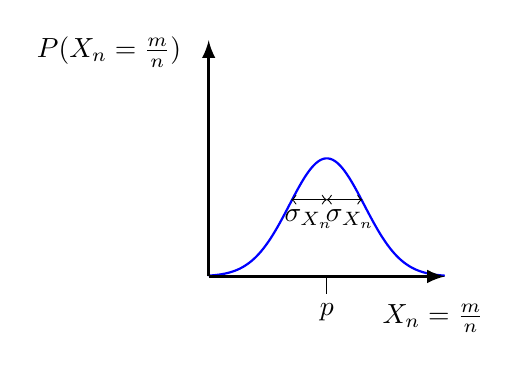
\begin{tikzpicture}[scale=1.5]
        \draw[blue, thick, smooth, samples = 100, domain=0:2, variable = \x] plot(\x, {exp(-((\x)-1)*((\x)-1)*5)});
        \draw[-latex, very thick] (0, 0) -- (2, 0);
        \draw[-latex, very thick] (0, 0) -- (0, 2);
        \node[left] at (-0.15, 1.9) {$P(X_n = \frac{m}{n})$};
        \node[below] at (1.9, -0.15) {$X_n = \frac{m}{n}$};
        \draw[] (1, 0) -- (1, -0.15);
        \node[below] at (1, -0.15) {$p$};
        \draw[<->] (1, 0.65) -- (1.3, 0.65);
        \draw[<->] (1, 0.65) -- (0.7, 0.65);
        \node[below] at (1.2, 0.65) {$\sigma_{X_n}$};
        \node[below] at (0.85, 0.65) {$\sigma_{X_n}$};
    \end{tikzpicture}
    
    \caption{Visualization of how $P(X_n)$. Since $\sigma_{X_n}$ (the width of the distribution) scales as $\frac{1}{\sqrt{n}}$, as $n$ grows, the distribution becomes more sharply peaked around $p$.}
    \label{fig47}
\end{figure}

\begin{ntheorem}{: Chebychev's Inequality}{}
    $P(\abs{X_n - p} > \delta) \leq \frac{1}{\sigma^2}p(1-p)\frac{1}{n}$. Note that this inequality can be generalized to random variables in general, but here it suffices to consider the inequality just for the case of $X_n$.
\end{ntheorem}
\begin{nproof}
    We have that:
    \begin{align*}
        P(\abs{X_n - p} > \delta) = \sum_{m: \abs{\frac{m}{n} - p} > \sigma}p_m \leq \sum_{m=0}^n \abs{\frac{\frac{m}{n} - p}{\sigma}}^2p_m = \frac{1}{\sigma^2}\sum_{m=0}^n \left(\frac{m}{n} - p\right)^2p_m &= \frac{1}{\sigma^2}\text{Var}(X_n) 
        \\ &= \frac{1}{\sigma^2}p(1-p)\frac{1}{n}.
    \end{align*}
    where in the first inequality we use the fact that $\abs{\frac{\frac{m}{n} - p}{\sigma}}^2 \geq 1$ and we hence add non-negative terms to the sum, and in the second to last equality we invoke the definition of the variance. \qed
\end{nproof}
\noindent With the machinery of basic probability established, we move to the proof of the Weierstrass theorem.

\begin{nproof}
    Take $p = x \in [0, 1]$. We then have that $p_m = \binom{n}{m}x^m(1-x)^{n-m}$. Let $P_n(x) = Ef(x_n) = \sum_{m=0}^n f(\frac{m}{n})p_m$ (why? as we take $n$ large, we have that $x_n \rightarrow x$, so $f(x_n) \rightarrow f(x)$, showing that $P_n(x)$ approximates $f(x)$ well). We note that $\sum_{m=0}^n f(\frac{m}{n})p_m$ is a polynomial in $x$ of degree $n$. This is our candidate for a uniformly convergent polynomial. We then have that:
    \begin{align*}
        f(x) - P_n(x) = \sum_{n=0}\left(f(x) - f\left(\frac{m}{n}\right)\right)p_m
    \end{align*}
    We will show that this is small by dividing it into two parts. For $\sigma > 0$, we have that:
    \begin{align*}
        \abs{f(x) - P_n(x)} &\leq \sum_{m: \abs{\frac{m}{n} - x} \leq \sigma} \abs{f(x) - f\left(\frac{m}{n}
        \right)}p_m + \sum_{m: \abs{\frac{m}{n} - x} > \sigma}\abs{f(x) - f\left(\frac{m}{n}\right)}p_m
        \\ &\leq \sum_{m: \abs{\frac{m}{n} - x} \leq \sigma} \abs{f(x) - f\left(\frac{m}{n}
        \right)}p_m + \sum_{m: \abs{\frac{m}{n} - x} > \sigma}2Mp_m
    \end{align*}
    where $M = \sup\set{f(x): x \in [0, 1]}$. Let $\e > 0$. we choose $\delta > 0$ such that $\abs{x - y} < \delta$ implies $\abs{f(x) - f(y)} < \frac{\e}{2}$. This choice is possible by the uniform continuity of $f$ (it is a continuous (polynomial) function on a compact set ($[0, 1]$)). Then, for the first term above we have that:
    \begin{align*}
        \sum_{m: \abs{\frac{m}{n} - x} \leq \sigma} \abs{f(x) - f\left(\frac{m}{n}
        \right)}p_m \leq \frac{\e}{2}\sum_{m=0}^n p_m = \frac{\e}{2}.
    \end{align*}
    For the second term, we apply Chebychev's inequality to get:
    \begin{align*}
        \sum_{m: \abs{\frac{m}{n} - x} > \sigma}2Mp_m \leq 2M\frac{1}{\delta^2}\frac{x(1-x)}{n}.
    \end{align*}
    Since $x(1-x) \leq \frac{1}{4}$ for $x \in [0, 1]$ we have:
    \begin{align*}
        \sum_{m: \abs{\frac{m}{n} - x} > \sigma}2Mp_m \leq 2M\frac{1}{\delta^2}\frac{x(1-x)}{n} \leq \frac{M}{2\delta^2}\frac{1}{n}.
    \end{align*}
    Now, choose $n$ such that $n > N \geq \frac{4\delta^2}{M\e}$. We then have that:
    \begin{align*}
        \frac{M}{2\delta^2}\frac{1}{n} < \frac{\e}{2}
    \end{align*}
    Then, we have that:
    \begin{align*}
        \abs{f(x) - P_n(x)} \leq \frac{\e}{2} + \frac{\e}{2} = \e
    \end{align*}
    which proves the claim. \qed
\end{nproof}
\noindent Our conclusion is that $P_n(x)$ is very close to $f(x)$. In the above proof, we split up the sum into two parts, and used different methods to obtain nice estimates/bounds on each. The next topic we will look at is generalizing this theorem; we will be building up to Rudin 7.32 (Stone-Weierstrass).

\setcounter{rudin}{27}

\begin{definition}{Algebras}{7.28a}
    Let $\A$ be a set of functions $f: E \mapsto \CC$ (or $\RR$). Then, $\A$ is an \textbf{algebra} if for all $f, g \in \A$ and for all $c \in \CC$, $f + g \in \A$, $fg \in \A$, and $cf \in \A$. 
\end{definition}

\begin{nexample}{}{}
    Let $E = [0, 1]$ and let $\A = \mathbb{P}$ be the set of polynomials on $[0, 1]$. Then, $\A$ is an algebra as the sum and product of two polynomials is also a polynomial, and a constant times a polynomial is a polynomial.
\end{nexample}

\setcounter{rudin}{27}

\begin{definition}{Uniformly Closed Algebras and Uniform Closure}{7.28b}
    We say that an algebra $\A$ is \textbf{uniformly closed} if $f_n \in \A$ and if $f_n \rightarrow f$ uniformly on $E$, then $f \in A$. In other words, the uniform limit of sequences of functions in the algebra is contained in the algebra. The \textbf{uniform closure} of $\A$ is then defined as $\mathcal{B} = \set{f: E \mapsto \CC: \exists f_n \in \A \text{ such that } f_n \rightarrow f \text{ uniformly}}$. 
\end{definition}

\begin{nexample}{}{}
    $\mathbb{P}$ in the above example is not closed, as the uniform limit of a polynomial is not necessarily a polynomial. $\C([0, 1])$ is uniformly closed as the limit of uniform and continuous functions are closed and bounded. $\C([0, 1])$ is also the uniform closure of $\mathbb{P}$ by the Weierstrass theorem (Theorem \ref{thm:7.26}). 
\end{nexample}

\begin{theorem}{}{7.29}
    The uniform closure $\mathcal{B}$ (sometimes denoted $\overline{\A}$) of an algebra $\A$  of bounded functions is a uniformly closed algebra. Note that $\A$ has a metric $d(f, g) = \sup_{x \in E}\abs{f(x) - g(x)} = \norm{f - g}$ and uniform convergence is equivalent to convergence in this metric.
\end{theorem}

\begin{nproof}
    Suppose $f, g \in \mathcal{B}$ and $c \in \CC$. Then, there exsits $\set{f_n}, \set{g_n} \subset \A$ such that $f_n \rightarrow f$ uniformly and $g_n \rightarrow g$ uniformly (that is, $\norm{f - f_n} \rightarrow 0$ and $\norm{g - g_n} \rightarrow 0$). We then have that:
    \begin{align*}
        f_n + g_n &\rightarrow f + g \text{ uniformly,}
        \\ fng_n &\rightarrow fg \text{ uniformly,}
        \\ cf_n &\rightarrow cf \text{ uniformly.}
    \end{align*}
    Note that the first two lines above correspond to Rudin problems 7.2 and 7.3 respectively (these are left as exercises to the reader). We conclude that $f+g, fg, cg \in \mathcal{B}$ and hence $\mathcal{B}$ is an algebra. Furthermore, it is uniformly closed as it consists of $\A$ and all limit points of $\A$ (hence $\mathcal{B} = \overline{\A}$). \qed
\end{nproof}

\begin{definition}{Separating Points and Vanishing at No Point}{7.30}
    A set $\A$ consisting of functions $f: E \mapsto \CC$ \textbf{separates points} on $E$ if for all $x_1, x_2$ in $E$ with $x_1 \neq x_2$, there exists $f \in \A$ such that $f(x_1) \neq f(x_2)$. In other words, there are enough functions in the set such that whatever pair of points we choose, we can always find distinct function values at these points. We say that $\A$ \textbf{vanishes at no point} in $E$ if for all $x \in E$, there exists $f \in \A$ such that $f(x) \neq 0$.
\end{definition}

\begin{nexample}{}{}
    \begin{enumerate}
        \item The set of polynomials $\mathbb{P}$ on $[-1, 1]$ separates points and vanishes at no point.
        \item The set of even polynomials on $[-1, 1]$ vanishes at no point but does not separate points (as for any $x \in (0, 1]$ and even polynomial $f$, $f(x) = f(-x)$).
        \item The set of odd polynomials on $[-1, 1]$ separates points, but all odd polynomials vanish at zero.
    \end{enumerate}
\end{nexample}

\setcounter{rudin}{31}

\begin{theorem}{Stone-Weierstrass}{7.32}
    The uniform closure of any algebra $\A$ of real continuous functions on a compact set $K$ which separates points and vanishes at no point is $\C(K)$ (i.e. the set of all continuous functions on $K$).
\end{theorem}
\noindent In other words, the above theorem tells us that given $\A$ that separates points and vanishes at no point on compact $K$, we can generate a sequence that uniformly converges to any continuous function on $K$. Note that the above theorem gives the Weierstrass theorem as a special case. Take $[a, b]$ and $\A = \mathbb{P}$ to be the polynomials on $[a, b]$. Then, $\mathbb{P}$ separates points and vanishes at no point, so according to the theorem, the uniform closure of $\mathbb{P}$ is all continuous functions on $[a, b]$. 

\begin{theorem}{Complex Stone-Weierstrass}{7.33}
    Let $\A$ be a set of real complex functions on a compact set $K$ which separates points and vanishes at no point. Furthermore, suppose that $\A$ is self adjoint, that is, if $f \in \A$, then $\overline{f} \in \A$ (where $\overline{f}(x) = \overline{f(x)}$). Then, the uniform closure of $\A$ is $\C(K)$. 
\end{theorem}

\noindent We establish three ingridients necessary for our proof of the Stone-Weierstrass theorem.

\begin{nlemma}{ 1}
    Let $\A$ be an algebra of real, continuous functions on a compact set $K$. Then, if $f \in \overline{\A}$, then $\abs{f} \in \overline{\A}$. 
\end{nlemma}

\begin{nproof}
    Let $f \in \overline{\A}$ and $M = \sup_{x \in K}\abs{f(x)}$. This $M$ is finite. Let $\e > 0$. By Theorem \ref{thm:7.26}, there exists a polynomial $\tilde{P}_n$ duch that:
    \begin{align*}
        \sup_{\abs{y} \leq M}\abs{\tilde{P}_n(y) - \abs{y}} < \frac{\e}{2}.
    \end{align*}
    Then, let $P_n(y) = \tilde{P}_n(y) - \tilde{P}_n(0) = \sum_{j=1}^n c_jy^j$. We then have that:
    \begin{align*}
        \abs{P_n(y) - \abs{y}} \leq \abs{\tilde{P}_n(0) - \abs{0}} + \abs{\tilde{P}_n(y) - \abs{y}} < \frac{\e}{2} + \frac{\e}{2} = \e
    \end{align*}
    Also, $P_n(f) = \sum_{j=1}^n c_jf^j \in \overline{\A}$ as $f \in \overline{\A}$ and hence sums/products of $f$ will be in the algebra. Note that the constant function may or may not be in the algebra, which is the reason why we define $P_n$ with the constant term left out (by subtracting $\tilde{P}_n(0)$ from $\tilde{P}_n(y)$). Moreover, we have that $\sup_{x \in K}\abs{P_n(f)(x) - \abs{f(x)}} < \e$ as $\abs{P_n(y) - \abs{y}} < \e$ for any $\abs{y} \leq M$ (since $\abs{f(x)} \leq M$ for all $x \in K$). Hence, $\abs{f} \in \overline{\A}$. \qed
\end{nproof}

\begin{nlemma}{ 2}
    For $\overline{\A}$ as in the previous Lemma (where $\overline{\A}$ is the uniform closure of a set of real, continuous functions on compact $K$), if $f_1, \ldots, f_n \in \overline{\A}$, then $\max\set{f_1, \ldots, f_n} \in \overline{\A}$ and $\min\set{f_1, \ldots, f_n} \in \overline{\A}$. 
\end{nlemma}

\begin{nproof}
    It suffices to consider the case where $n = 2$. For this we use that:
    \begin{align*}
        \max\set{f_1, f_2} &= \frac{1}{2}(f_1 + f_2) + \frac{1}{2}\abs{f_1 - f_2}
        \\ \min\set{f_1, f_2} &= \frac{1}{2}(f_1 + f_2) - \frac{1}{2}\abs{f_1 - f_2}
    \end{align*}
    Then, as $\overline{\A}$ is an algebra, we have that $\frac{1}{2}(f_1 + f_2) \pm \frac{1}{2}\abs{f_1 - f_2} \in \overline{\A}$ by Lemma 1. \qed
\end{nproof}
\noindent As a quick verification of the above formulas for the max/min over $\set{f_1, f_2}$, we can WLOG consider the case where $f_1 \geq f_2$:
\begin{align*}
    \frac{1}{2}(f_1 + f_2) + \frac{1}{2}\abs{f_1 - f_2} = &\frac{1}{2}(f_1 + f_2) + \frac{1}{2}(f_1 - f_2) = f_1 = \max\set{f_1, f_2}
    \\ \frac{1}{2}(f_1 + f_2) - \frac{1}{2}\abs{f_1 - f_2} = &\frac{1}{2}(f_1 + f_2) - \frac{1}{2}(f_1 - f_2) = f_2 = \min\set{f_1, f_2}
\end{align*}

\setcounter{rudin}{30}

\begin{theorem}{}{7.31}
    If an algebra $\A$ of functions on $E$ separates points and vanishes at no point, then given any $x_1, x_2 \in E$ with $x_1 \neq x_2$ and constants $c_1, c_2$, there exists $f \in \A$ such that $f(x_1) = c_1$ and $f(x_2) = c_2$. 
\end{theorem}

\begin{nproof}
    By hypothesis, there exists $g \in A$ such that $g(x_1) \neq g(x_2)$ (as $\A$ separates points). Furthermore, there exists $h, k \in \A$ such that $h(x_1) \neq 0$ and $k(x_2) \neq 0$ as $\A$ vanishes at no point. Let:
    \begin{align*}
        u(x) &= (g(x) - g(x_1))k(x)
        \\ v(x) &= (g(x) - g(x_2))h(x)
    \end{align*}
    Then, $u(x_1) = 0$ and $u(x_2) \neq 0$, and $v(x_1) \neq 0$ and $v(x_2) = 0$. Note that the $k, h$s are necessary to include in the above definitions of $u, v$ to ensure that $u, v$ lie in our algebra; $g(x) - g(x_i)$ may not be in $\A$ if the constant functions are not in $\A$. Now, let:
    \begin{align*}
        f(x) = c_1\frac{v(x)}{v(x_1)} + c_2\frac{u(x)}{u(x_2)}
    \end{align*}
    which is a meaningful definition as $v(x_1) \neq 0$ and $u(x_2) \neq 0$. Since $\A$ is an algebra, $f \in \A$. Furthermore, we have that:
    \begin{align*}
        f(x_1) = c_1\frac{v(x_1)}{v(x_1)} + c_2\frac{u(x_1)}{v(x_2)} = c_1 + 0 = c_1
    \end{align*}
    and identically $f(x_2) = c_2$, proving the claim. \qed
\end{nproof}

\noindent We now proceed into the proof of Theorem \ref{thm:7.32}. As a brief refresher, we have an algebra $\A$ of continuous real functions on a compact set $K$, which vanishes points and separates at no point. We wish to show that for all continuous functions $f: K \mapsto \RR$ and for all $\e > 0$, there exists $h \in \mathcal{B} = \overline{\A}$ such that $\norm{h - f} < \e$. 
